\newpage
\section{Appendix: Extended Results}
\label{app:results}

\subsection{Linear versus non-linear}

We expect CAREFL to do well on the linear PGM problem as the structure of the PGM matches CAREFL's inductive bias: affine transformations of a fixed base distribution. But since these assumptions are restrictive, we expect CAREFL to perform poorly on the non-linear PGM problem. \cam{The results (Figures~\ref{fig:swd-linear-v-nonlinear} and~\ref{fig:counterfactual-linear-v-nonlinear}) bear this out: on the linear benchmarks CAREFL is the strongest method on counterfactual queries---abduction through its exactly-matched affine inverse is nearly exact---although Static and the universal flow lead on interventional queries; on the nonlinear benchmarks CAREFL falls behind the structured CNFs on both. Dynamic conditioning is close to Static on the nonlinear graphs (interventional SWD within $15\%$) but clearly worse on the linear ones (${\sim}2.6\times$ on interventional queries), where the strong linear dependence between blocks makes the residual bias of the minibatch per-block coupling largest (Section~\ref{sec:chain-stiffness}).}

\begin{figure*}[hbt!]
    \centering
    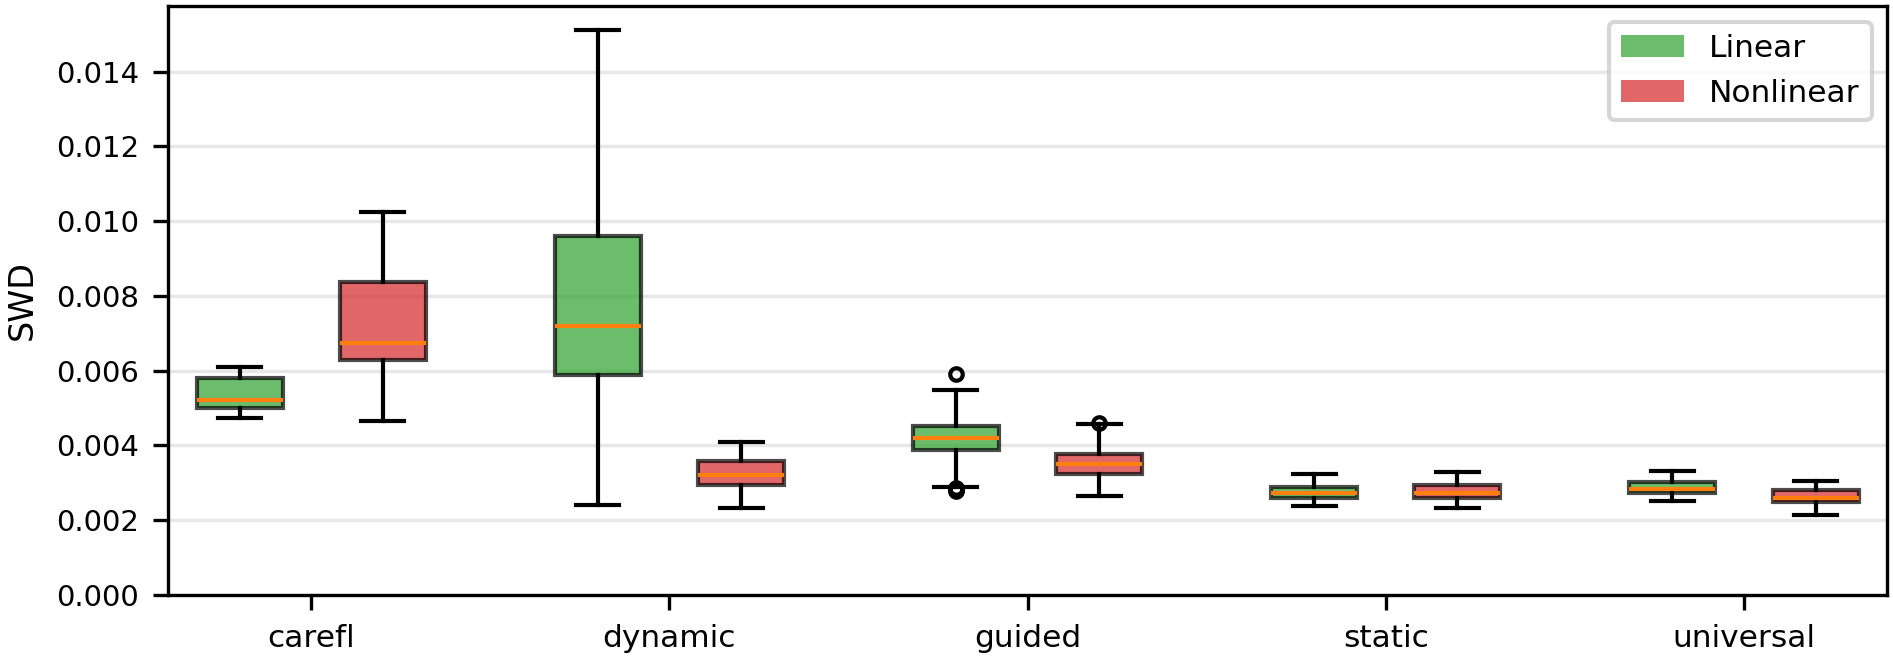
\includegraphics[width=\textwidth]{images/experimental_figures/pgm_type_comparison_swd_task_causal_conditional.png}
    \caption{\textbf{Interventional Query Results.} Sliced Wasserstein Distance for interventional distributions $p(y \mid \mathrm{do}(x))$ on linear and nonlinear PGMs (these coincide with the observational conditionals $p(y \mid x)$ for the evaluated query family; see Section~\ref{sec:experiments}). Results aggregated over 5 PGM seeds and 5 learner seeds.}
    \label{fig:swd-linear-v-nonlinear}
\end{figure*}

\begin{figure*}[hbt!]
    \centering
    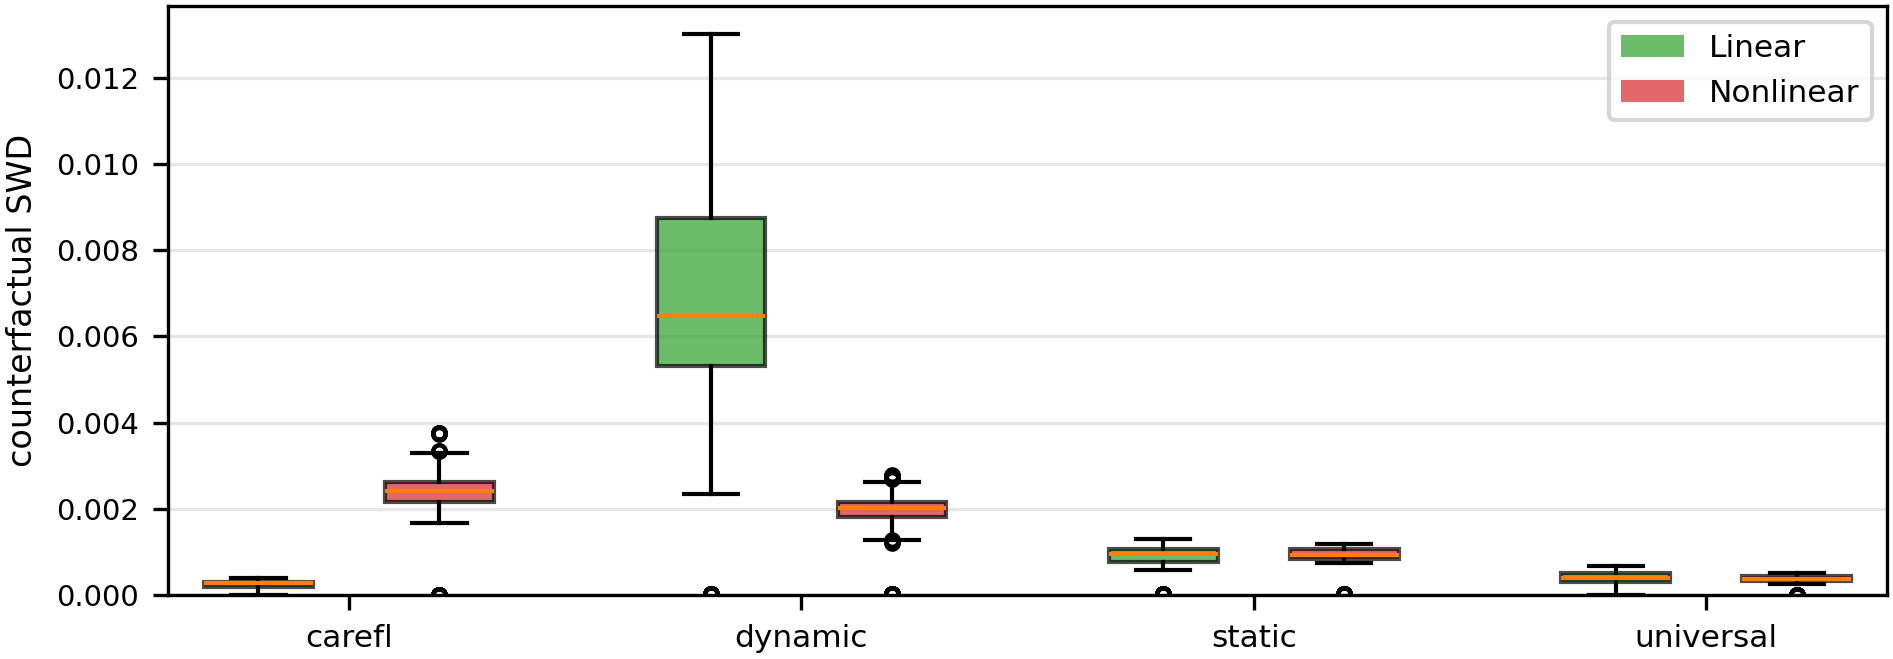
\includegraphics[width=\textwidth]{images/experimental_figures/pgm_type_comparison_counterfactual_swd_task_causal_conditional.png}
    \caption{\textbf{Counterfactual Query Results.} Sliced Wasserstein Distance for counterfactual distributions on linear and nonlinear PGMs. Aggregated over 5 PGM seeds and 5 learner seeds.}
    \label{fig:counterfactual-linear-v-nonlinear}
\end{figure*}

\subsection{KL divergence on linear-Gaussian causal queries}
\label{app:kl-linear}

On the linear-Gaussian benchmarks the ground-truth conditionals are available in closed form, so the causal queries can additionally be scored by KL divergence, which puts the (deliberately small) normalized SWD values of Section~\ref{sec:experiments} on a calibrated scale. Table~\ref{tab:linear4-kl} reports median scores on the $4$-node linear benchmark, aggregated over conditional causal queries, $5$ PGM seeds and $5$ learner seeds. \cam{Among the methods that define a tractable conditional density, KL and SWD agree on interventional queries that Static and the universal flow are best (near-tied by SWD; KL favors the universal flow) and Dynamic is worst; guided sampling defines no conditional density for most queries, so its KL is omitted. On counterfactuals SWD ranks CAREFL first, then the universal flow and Static, with Dynamic far behind. The log-ratio column (see below) instead puts Static and the universal flow nearest zero and CAREFL and Dynamic at ${\sim}0.2$; it measures agreement of the interventional densities, not counterfactual accuracy, so the two need not agree.}

A remark on what the counterfactual columns measure. Our factuals are \emph{fully observed}, so by Remark~\ref{rem:density-scope} each counterfactual is a point mass and has no density of its own. The ``Cf.'' entries are therefore \emph{not} divergences between counterfactual distributions: each model evaluates the density of its own \emph{mutilated (interventional)} distribution at the counterfactual point, and the reported score is the mean log-ratio of the true and learned interventional densities over the factual population---a calibration diagnostic asking whether the two mutilated models agree along the manifold where counterfactuals land. Read this way, the column is consistent with Remark~\ref{rem:density-scope}; \cam{it is a calibration check, and it does not rank methods by counterfactual accuracy.}

\begin{table}[h]
\centering
\caption{\textbf{KL divergence versus SWD on the $4$-node linear-Gaussian benchmark} (causal task, conditional queries; median over queries, $5$ PGM seeds and $5$ learner seeds). ``Int.''\ denotes interventional queries; ``Cf.''\ entries are interventional-density log-ratios evaluated at the counterfactual points (see text---the counterfactual itself is a point mass under full observation, Remark~\ref{rem:density-scope}). \cam{Being a mean log-ratio rather than a divergence, a Cf.\ entry can be slightly negative.} KL corroborates the SWD ordering of the density-bearing methods; guided sampling has no tractable conditional density, so KL is unavailable for it.}
\label{tab:linear4-kl}
\begin{tabular}{lrrrr}
\toprule
\textbf{Method} & \textbf{Int.\ SWD} & \textbf{Int.\ KL} & \textbf{Cf.\ SWD} & \textbf{Cf.\ KL} \\
\midrule
Static    & 0.0027 & 0.055 & 0.0009 & $-0.024$ \\
Universal & 0.0028 & 0.025 & 0.0004 & 0.023 \\
Guided    & 0.0042 & ---   & ---    & ---   \\
CAREFL    & 0.0052 & 0.221 & 0.0003 & 0.214 \\
Dynamic   & 0.0071 & 0.232 & 0.0065 & 0.200 \\
\bottomrule
\end{tabular}
\end{table}

\subsection{Learning the joint distribution: causal structure versus inference structure}

Is one direction (causal versus inference) better at learning the joint distribution than the other? No: for every flow-based method the two structures give joint SWDs within $3\%$ of each other (e.g.\ Static $1.30$ vs.\ $1.32 \times 10^{-3}$), and CAREFL is $5\%$ lower with the inference structure, while remaining about twice the others' error in both (Figure~\ref{fig:nonlinear-joint}).

\begin{figure}[hbt!]
    \centering
    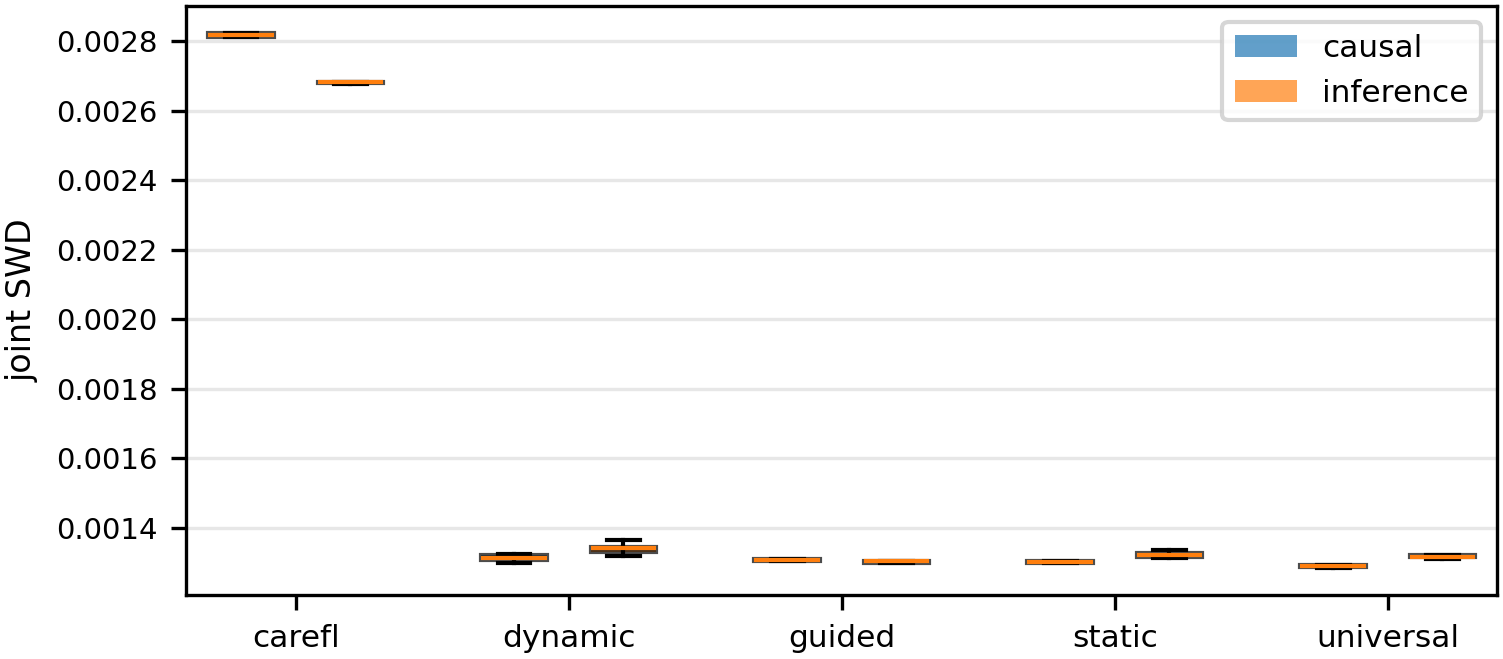
\includegraphics[width=0.8\textwidth]{images/experimental_figures/nonlinear/task_comparison_swd_joint.png}
    \caption{\textbf{Joint-distribution SWD by compiled structure} on the nonlinear $4$-node PGMs. For each method, the left box is the model trained with the causal structure and the right box the model trained with the inference structure; each box shows the spread over $5$ learner seeds, each averaged over $5$ PGM seeds.}
    \label{fig:nonlinear-joint}
\end{figure}

\subsection{Granular PGM metrics}

Figures~\ref{fig:causal-nonlinear-pgm-queries} and~\ref{fig:inference-nonlinear-pgm-queries} break the aggregated nonlinear results of Figure~\ref{fig:pgm-results} down by query.

\begin{figure}[hbt!]
    \centering
    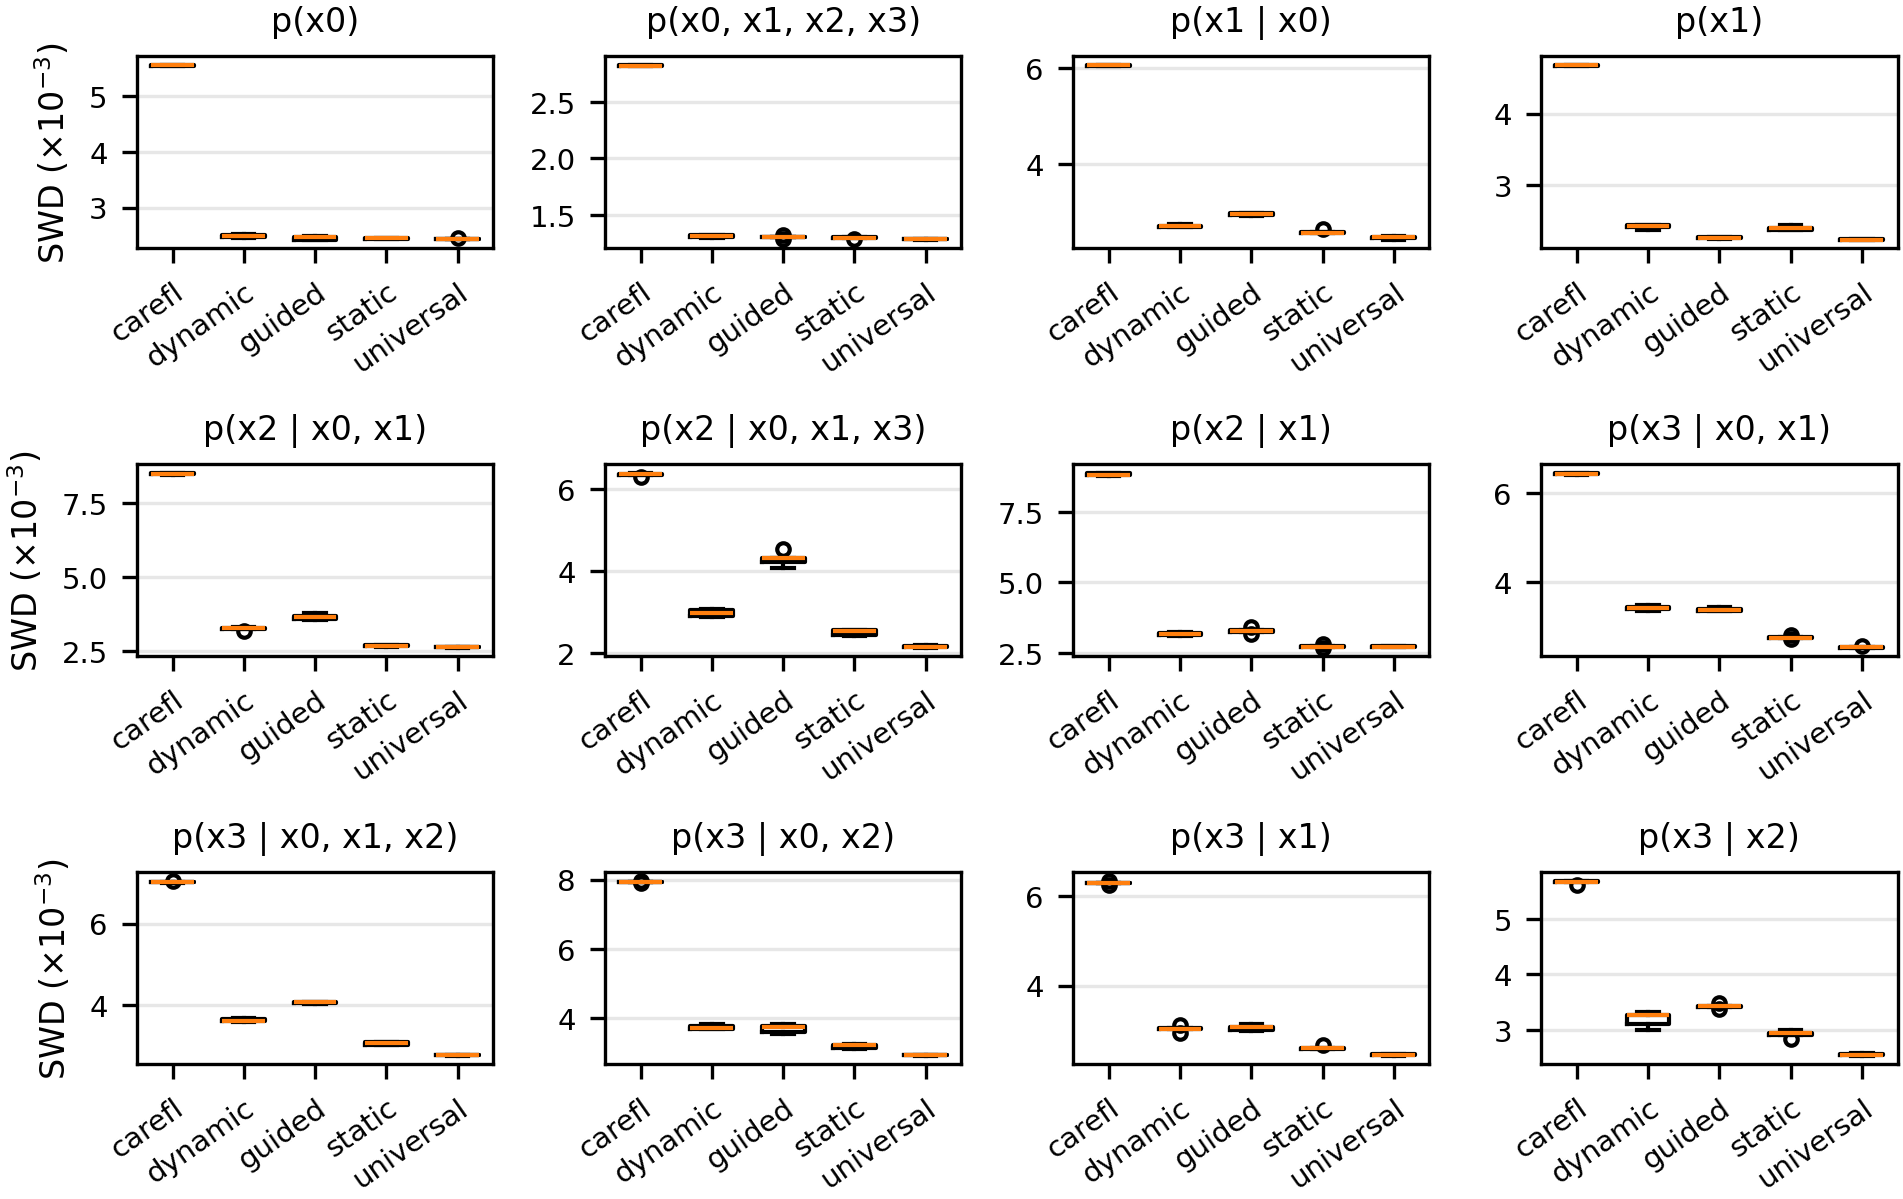
\includegraphics[width=\textwidth]{images/experimental_figures/nonlinear/final_box_swd_pgms_all_task_causal_queries_all.png}
    \caption{\textbf{Per-query breakdown of Figure~\ref{fig:pgm-results}a} (causal alignment, nonlinear $4$-node PGMs). One panel per query; each box shows the spread over $5$ learner seeds, each averaged over the $5$ PGM seeds. Read for the ranking of methods within each panel; scales differ between panels.}
    \label{fig:causal-nonlinear-pgm-queries}
\end{figure}

\begin{figure}[hbt!]
    \centering
    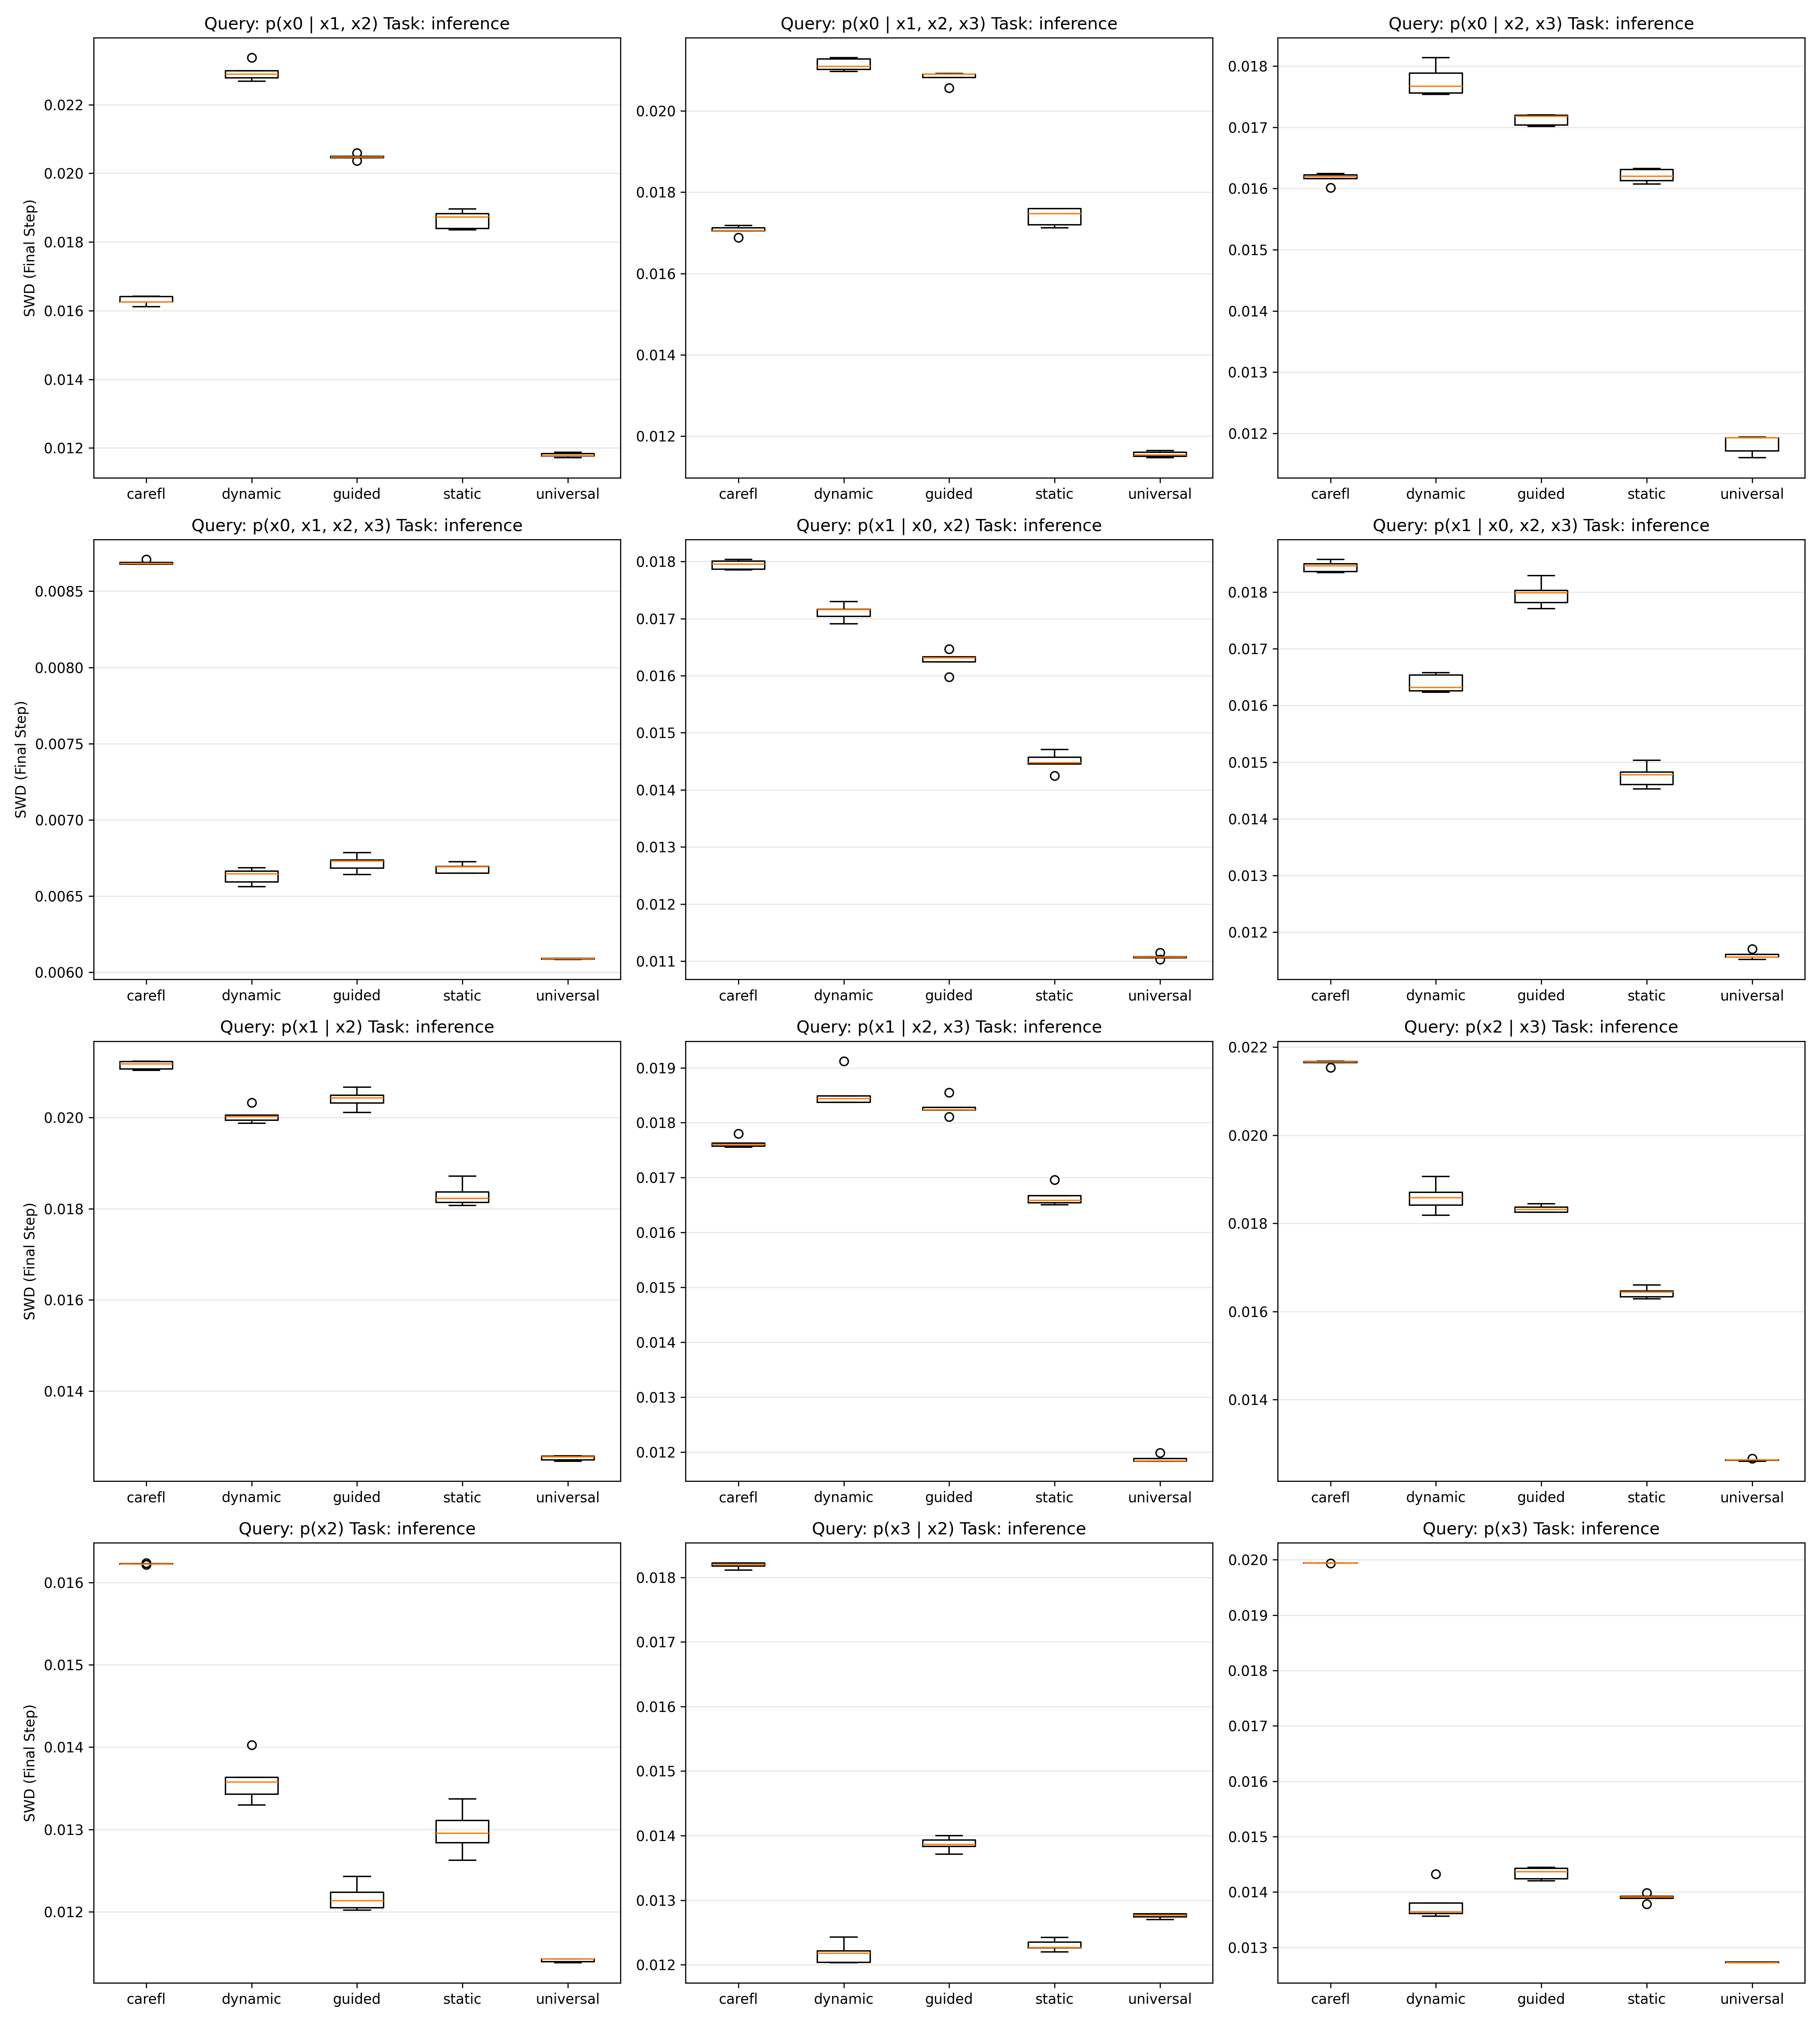
\includegraphics[width=\textwidth]{images/experimental_figures/nonlinear/final_box_swd_pgms_all_task_inference_queries_all.png}
    \caption{\textbf{Per-query breakdown of Figure~\ref{fig:pgm-results}c} (inference alignment, nonlinear $4$-node PGMs). One panel per query; each box shows the spread over $5$ learner seeds, each averaged over the $5$ PGM seeds. Read for the ranking of methods within each panel; scales differ between panels.}
    \label{fig:inference-nonlinear-pgm-queries}
\end{figure}

\subsection{Scaling to $8$-node PGMs}

To check that the framework is not limited to very small graphs, we repeat the inference evaluation on random $8$-node nonlinear PGMs ($5$ PGM seeds $\times$ $5$ learner seeds). Figure~\ref{fig:inference-n8} shows that the qualitative picture is unchanged from $n=4$\cam{: Universal is most accurate ($3.4 \times 10^{-3}$, mean over runs), static conditioning follows closely ($3.9$), and guidance, CAREFL and dynamic conditioning form a second group ($4.8$--$5.0$), the same ordering as on the $4$-node inference queries. Seed-to-seed spread is small ($\leq 0.3 \times 10^{-3}$), so the gaps between the two groups are well resolved.} This is consistent with our central finding---on well-sampled graphs, structure is a competitive but not dominant choice, and its advantage is most visible under limited data (Appendix~\ref{sec:sample-efficiency}). The binding constraint on scaling further is \emph{evaluation}, not training: generating MCMC ground truth for every conditional query grows quickly with $n$ (Section~\ref{sec:future_work}).

\begin{figure}[hbt!]
    \centering
    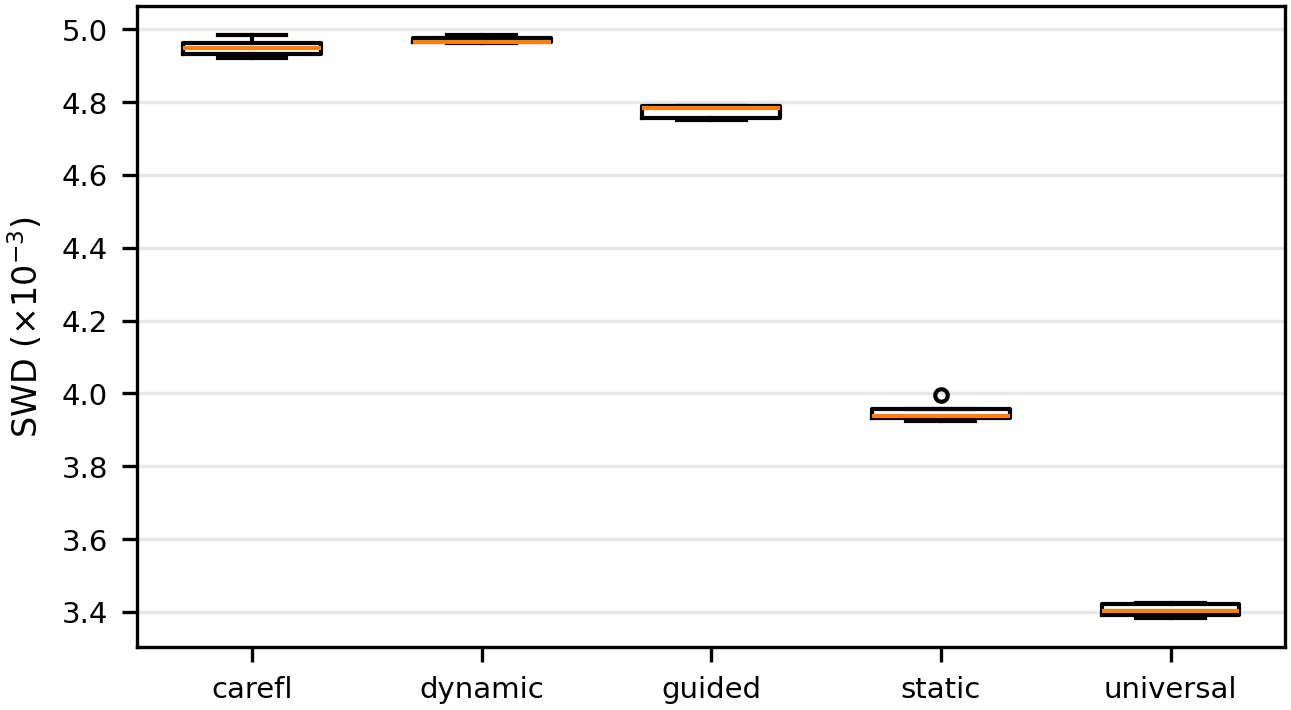
\includegraphics[width=0.7\textwidth]{images/experimental_figures/nonlinear8/final_box_swd_pgms_all_task_inference_queries_avg_conditional.png}
    \caption{\textbf{Inference on $8$-node nonlinear PGMs.} Normalized SWD on posterior queries, aggregated over conditional queries, $5$ PGM seeds and $5$ learner seeds. Universal is the structured spline flow of Section~\ref{sec:experiments}, the mechanism family that generates these PGMs. The structured (Static) flow remains competitive at $n=8$, matching the $n=4$ trend\cam{; note the $y$-axis does not start at zero}.}
    \label{fig:inference-n8}
\end{figure}

\subsection{MNIST}

\begin{figure*}[hbt!]
    \centering
    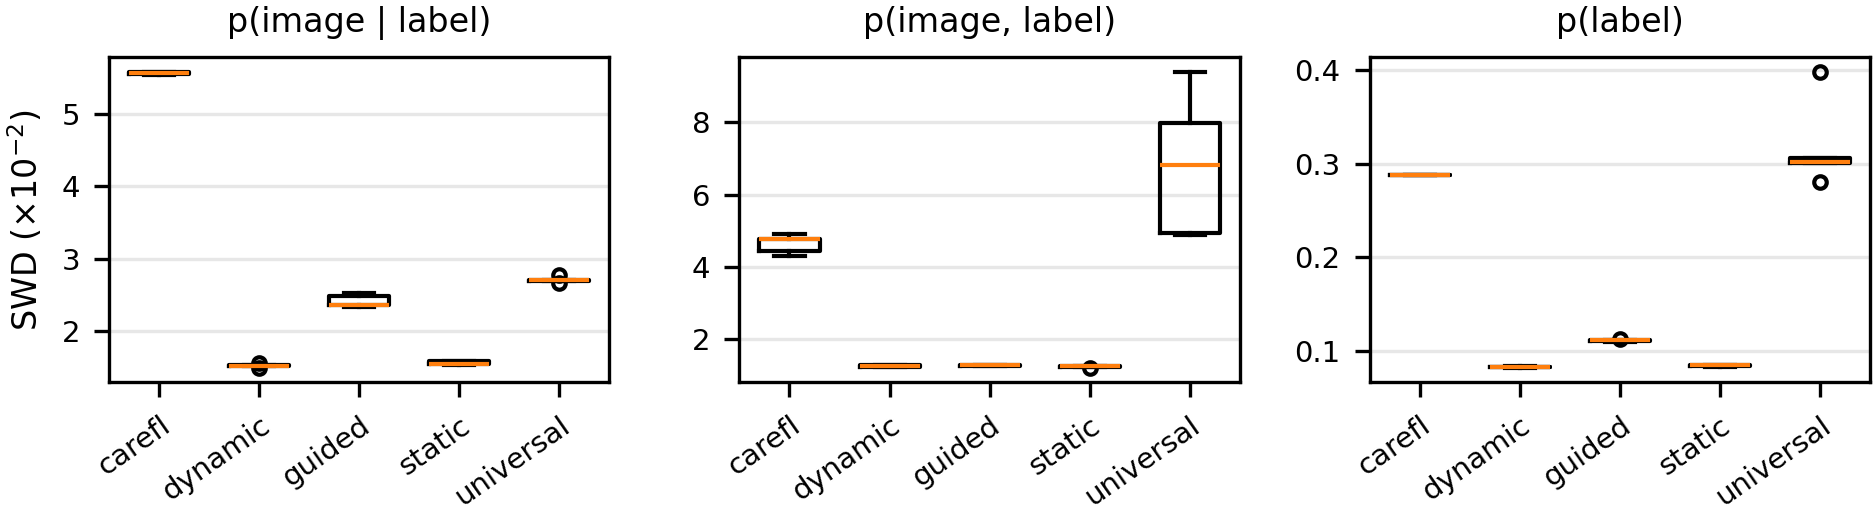
\includegraphics[width=\textwidth]{images/experimental_figures/mnist/final_box_swd_pgms_all_task_all_queries_all.png}
    \caption{\textbf{MNIST Results.} Sliced Wasserstein Distance across joint, marginal, and conditional distributions for the structure \texttt{labels}$\to$\texttt{images}. Aggregated over 5 seeds.}
    \label{fig:mnist-swd}
\end{figure*}

\begin{figure}[hbt!]
    \centering
    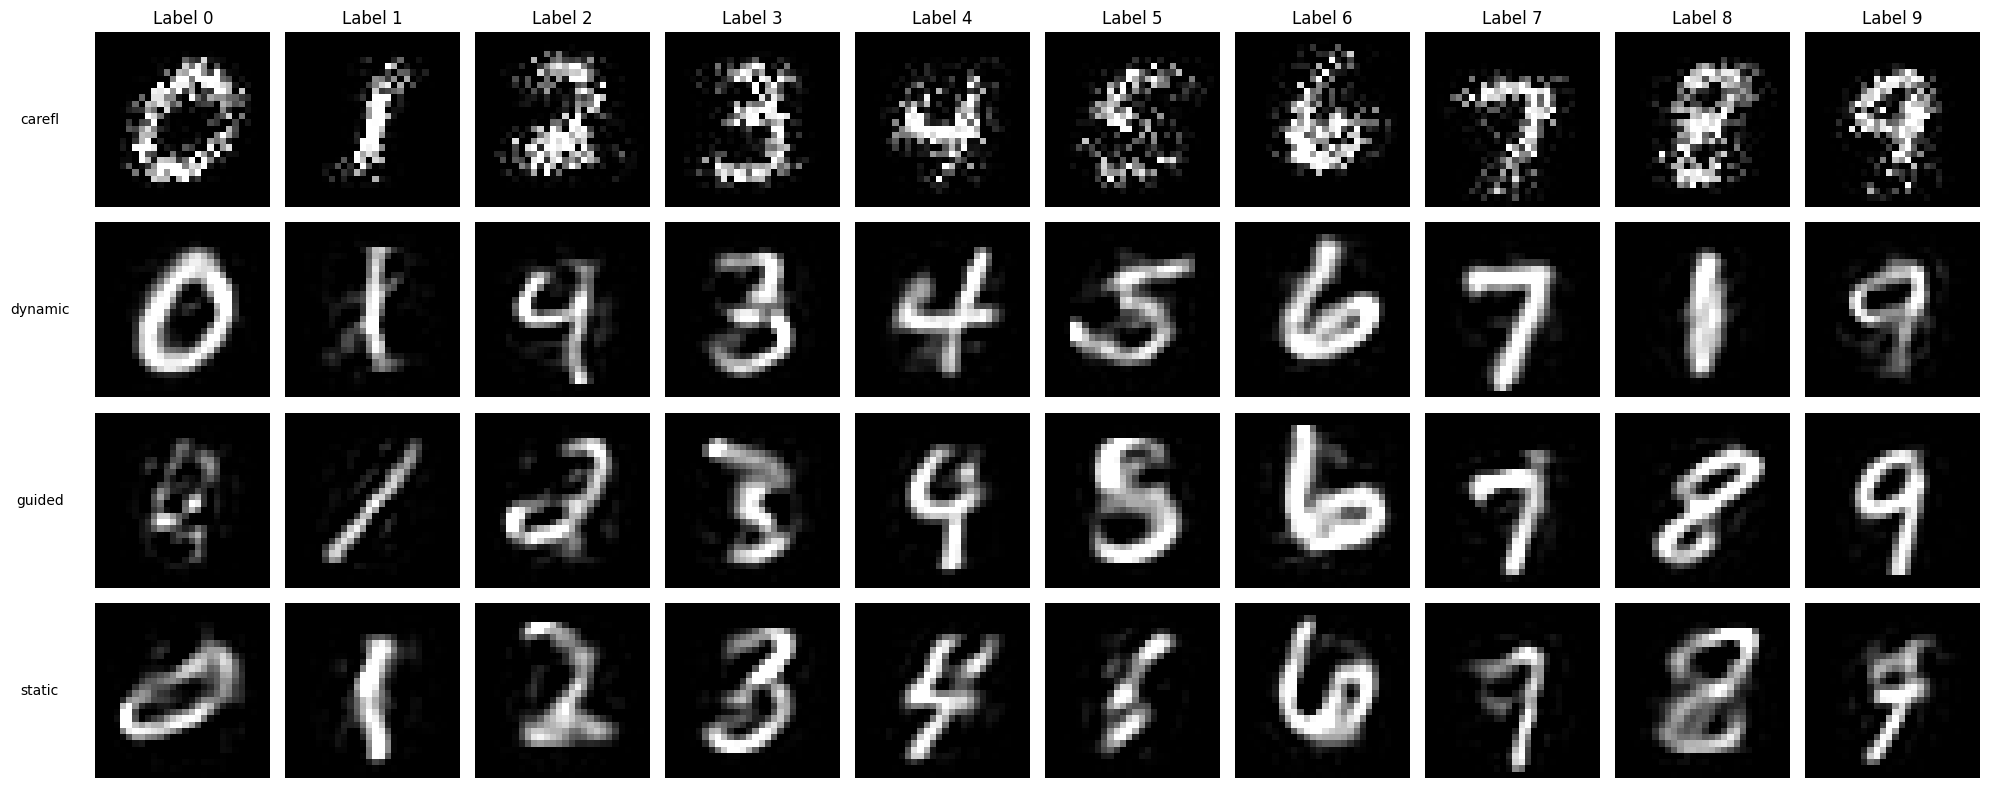
\includegraphics[width=\textwidth]{images/experimental_figures/mnist/mnist_samples1.png}
    \caption{Samples of $p(\text{image} \mid \text{label})$ from four of the MNIST models (rows: CAREFL, Dynamic, Guided, Static; columns: conditioning label), one learner seed.}
    \label{fig:mnist-sample1}
\end{figure}

\begin{figure}[hbt!]
    \centering
    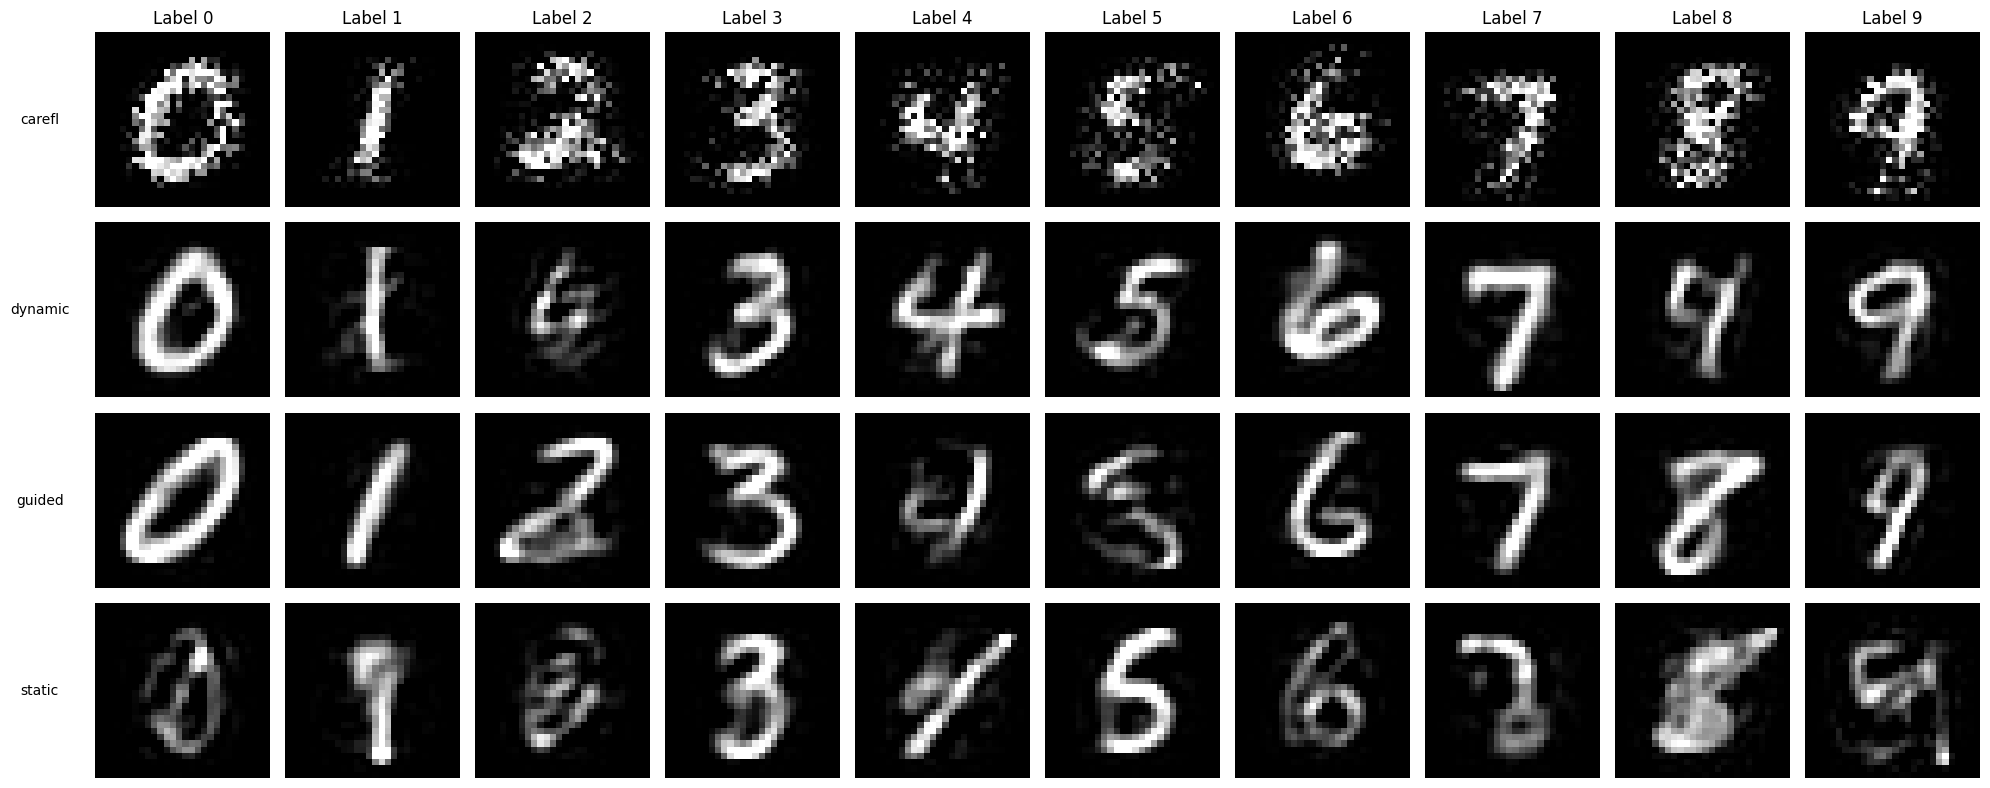
\includegraphics[width=\textwidth]{images/experimental_figures/mnist/mnist_samples2.png}
    \caption{Samples of $p(\text{image} \mid \text{label})$ from four of the MNIST models (rows: CAREFL, Dynamic, Guided, Static; columns: conditioning label), one learner seed.}
    \label{fig:mnist-sample2}
\end{figure}

\begin{figure}[hbt!]
    \centering
    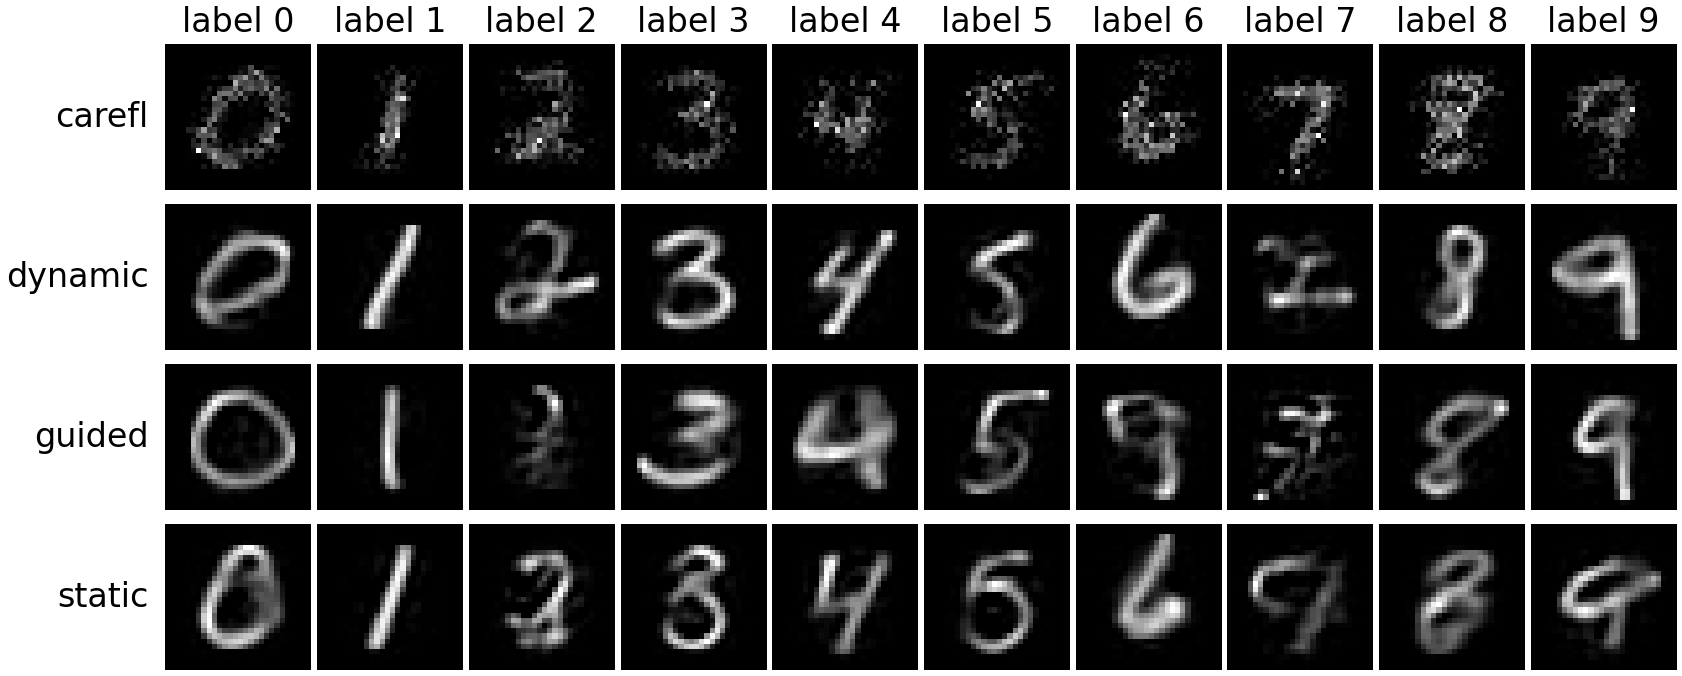
\includegraphics[width=\textwidth]{images/experimental_figures/mnist/mnist_samples3.png}
    \caption{Samples of $p(\text{image} \mid \text{label})$ from four of the MNIST models (rows: CAREFL, Dynamic, Guided, Static; columns: conditioning label), one learner seed.}
    \label{fig:mnist-sample3}
\end{figure}
